\section{The canonical target antichain}
\label{sec:universal}
We first isolate a fact about closed footprints and regular closed targets. This step is what permits an exact full-target conclusion from open arrangement cells.

\begin{lemma}[Interior witnesses]\label{lem:interior-witness}
Let $T=\overline{\operatorname{int}T}$ be a nonempty regular closed target and let $D_1,\ldots,D_n$ be closed sets whose boundaries have empty interior. For every $x\in T$ there is a point $y\in\operatorname{int}T$, away from all the boundaries, with $S(y)\subseteq S(x)$. For a finite disk family and triangular target, $y$ may be chosen rational.
\end{lemma}
\begin{proof}
For each $i\notin S(x)$, closedness gives an open neighborhood of $x$ disjoint from $D_i$. Intersect these finitely many neighborhoods to obtain an open set $U$ in which no new active label can appear. Regular closedness implies $U\cap\operatorname{int}T\ne\varnothing$. A finite union of disk boundaries and target edges has empty interior, so it cannot exhaust this nonempty open set. Choose $y$ outside it. The active labels of $y$ are all in $S(x)$. In the disk setting, the remaining open set contains rational points by density of $\mathbb Q^2$.
\end{proof}

For the first general statement, the avoidance assertion uses that the finitely many boundaries are closed with empty interior, hence nowhere dense. Disk circles and target edges satisfy this condition. No claim about arbitrary nonclosed sensing footprints is needed.

\begin{definition}
The \emph{target antichain} is
\[
\mathcal A_T(D)=\Min\{S(x):x\in T\}.
\]
The empty contact set is retained if realized. If it occurs, it is the unique minimal member. A witness for $A\in\mathcal A_T$ is a point $q_A\in T$ with $S(q_A)=A$.
\end{definition}

\begin{theorem}[Universal target certificate]\label{thm:universal}
For a finite closed-disk family and a regular closed triangular target, $\mathcal A_T$ is exactly the collection of inclusion-minimal labels of the two-dimensional target arrangement cells. Every member has a rational interior witness. For every downward-closed failure family $\F$ containing the empty set,
\begin{equation}\label{eq:universal-target}
T\subseteq R_{\F}\quad\Longleftrightarrow\quad
\mathcal A_T\cap\F=\varnothing.
\end{equation}
If $h$ target-edge segments are supplied, the certificate has $O((n+h)^2)$ members.
\end{theorem}
\begin{proof}
The finite collection of all realized masks has an inclusion-minimal member below every mask. If $A$ is such a minimal mask, apply \cref{lem:interior-witness} at a point realizing $A$. The resulting interior mask is a subset of $A$, so minimality forces equality. Conversely, if an interior-cell mask is minimal among interior-cell masks, a smaller realized mask would have an interior witness below it by the lemma, a contradiction. Thus the two minimal collections agree.

By \cref{prop:pointwise}, full target coverage means $S(x)\notin\F$ for every $x\in T$. Necessity of the right side is immediate from witnesses. For sufficiency, choose $A\subseteq S(x)$ in the antichain. If $S(x)\in\F$, downward closure would imply $A\in\F$, contradicting the right side. This proves \cref{eq:universal-target}.

For the size bound, refine the disk arrangement by the supporting lines of all target edges. With $n$ distinct positive-radius circles, adding circle $j$ creates at most $\max\{1,2(j-1)\}$ new regions. A newly added line meets the circles at most $2n$ times and the preceding $j-1$ lines at most $j-1$ times, so it creates at most $2n+j$ regions. Coincident curves can be removed for counting; repeated sensor labels are still preserved on each region. Zero-radius disks add no two-dimensional region. Consequently the total number of regions is at most
\begin{equation}\label{eq:arrangement-bound}
n^2-n+2+2nh+\frac{h(h+1)}2,
\end{equation}
where the harmless initial constant also bounds the $n=0$ case. Target membership and contact labels are constant on every open region of this refined arrangement. The number of minimal labels cannot exceed its number of regions.
\end{proof}

\begin{remark}
The quadratic bound counts the retained certificate, not the vertical bands sampled in its construction. It is inherited from ordinary arrangement complexity. No matching quadratic lower bound for this particular minimal-label family is asserted.
\end{remark}

\begin{proposition}[Irredundancy for all failure rules]\label{prop:irredundant}
Every member of $\mathcal A_T$ is necessary if a certificate consists of realized contact masks and is required to answer all downward-closed failure queries by testing those masks. In particular, deleting any one member can change an answer.
\end{proposition}
\begin{proof}
Fix $A\in\mathcal A_T$ and use $\F=2^A$. Then $A$ loses. Every other antichain member $B$ is not a subset of $A$, so $B\notin\F$. Testing all the remaining members would therefore accept although the witness $q_A$ fails. When $A=\varnothing$, its antichain has only that member and the same argument applies to the family allowing only the empty failure, $2^\varnothing=\{\varnothing\}$.
\end{proof}

This is minimality of the representation by realized masks. It is not a lower bound against every possible compressed circuit, geometric formula or data structure.\footnote{An irredundant list can still admit a shorter symbolic representation. We do not identify the number of listed cuts with an information-theoretic lower bound for all encodings.}

\begin{theorem}[Monotone relabeling]\label{thm:relabel}
Let $\gamma:2^{[n]}\to2^{[m]}$ preserve inclusion. The minimal target patterns after applying $\gamma$ to active sets are exactly
\begin{equation}\label{eq:relabel}
\Min\{\gamma(A):A\in\mathcal A_T\}.
\end{equation}
Each retained image inherits a witness from its preimage. Thus no new geometric computation is needed for contact deletion, fault-domain coarsening or monotone virtual-contact logic.
\end{theorem}
\begin{proof}
Every realized $S(x)$ contains some $A\in\mathcal A_T$, so $\gamma(S(x))$ contains $\gamma(A)$. Conversely every image $\gamma(A)$ is itself realized at $q_A$. Taking minimal members on both sides proves the equality and the witness assertion.
\end{proof}

For a permanent deletion set $F$, take $\gamma(S)=S\setminus F$. For a partition into domains, take $\gamma(S)$ to be the set of domains touched by $S$. For a contact represented by several primitive disk constraints, let its output bit be one exactly when all its primitive bits are one. This conjunction map is monotone and is used for uncertain placement in \cref{sec:uncertainty}.

\begin{corollary}[Exact deletion budgets]\label{cor:budgets}
For nonnegative contact deletion costs $c_i$, the minimum cost of a failure that destroys full target coverage is
\begin{equation}\label{eq:kappa}
\kappa_T(c)=\min_{A\in\mathcal A_T}\sum_{i\in A}c_i.
\end{equation}
It is attained by deleting a minimizing $A$, with failure witnessed at $q_A$. Full target coverage survives every deletion of cost at most $B$ if and only if $B<\kappa_T(c)$.
\end{corollary}
\begin{proof}
A deletion $F$ destroys coverage precisely when it contains a realized active set, and hence when it contains some antichain member. Nonnegative costs give $c(F)\ge c(A)$. Conversely deleting $A$ removes every active contact at its witness. The strict budget inequality follows because a deletion of cost exactly $\kappa_T(c)$ is allowed when $B$ reaches that value.
\end{proof}

For unit costs, the maximum guaranteed number of arbitrary contact losses is $\min_A|A|-1$, provided the target is initially covered. For a domain partition, apply \cref{thm:relabel} first and use one cost per domain. The case $\kappa_T=0$ is not rounded up: it means that no nonnegative budget guarantee holds, either because the target is already uncovered or because a zero-cost cut is available.

\begin{figure*}[tb]
\centering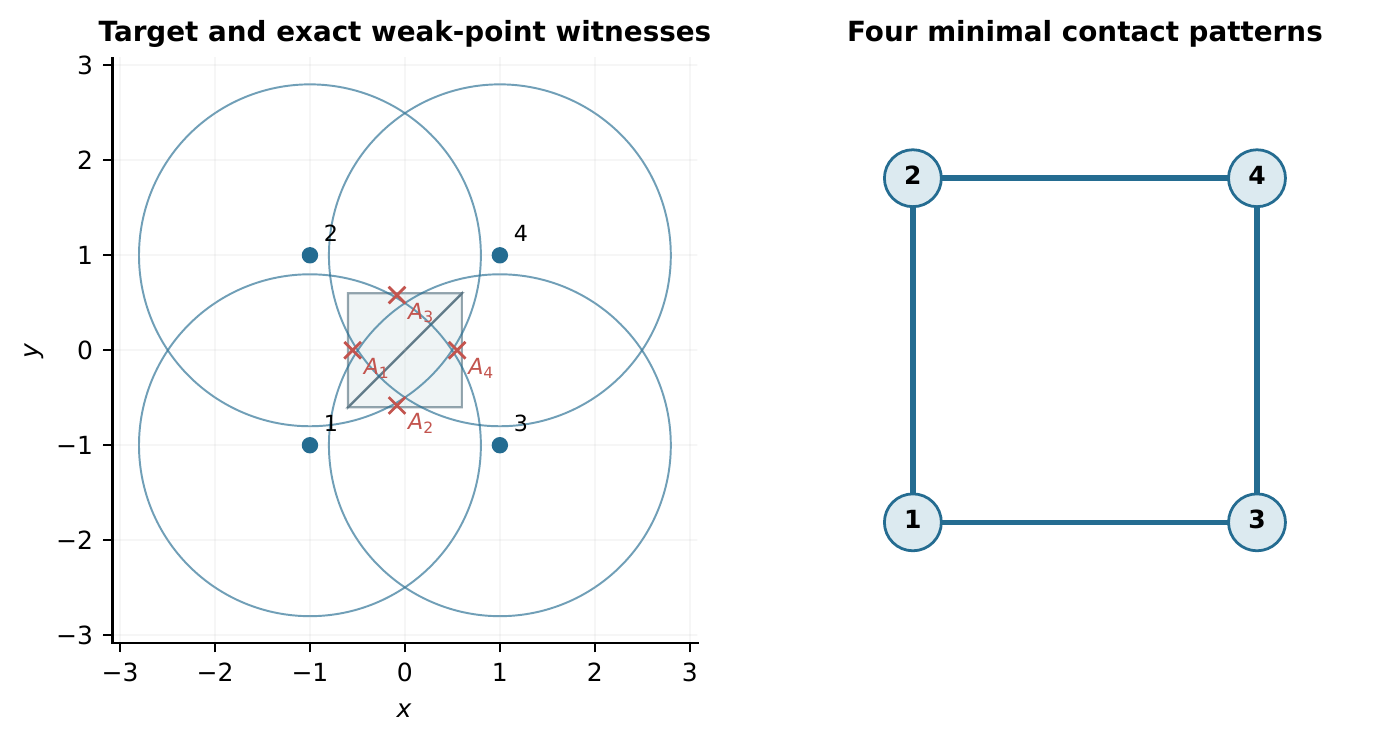
\includegraphics[width=\textwidth]{figures/target-patterns.png}
\caption{Target geometry with exact rational witnesses and the minimal cut graph of the four-contact panel. The witnesses and all four critical pair patterns are derived explicitly in \cref{sec:engineering}.}
\end{figure*}

